\section{Raspberry Pi}
\setauthor{Sebastian Egger}

Das Projekt beinhaltet einen Raspberry Pi 4, welcher als MQTT Broker dient. Auf diesem Raspberry Pi läuft unser Backend mit DotNet, Docker und Samba.
Der Raspberry Pi hat 4 Gigabyte RAM und eine 32 Gigabyte SSD. 
Die Verbindung zwischen dem Raspberry und der SSD wird mit einem USB-Adapter hergestellt. 
Die SSD wurde unter dem Raspberry mittels einer Platine und Schrauben befestigt. 
Der Raspberry braucht mindestens 3 und maximal 11 Watt. 
\cite{RASPPI}

\begin{figure}[H]
    \centering
    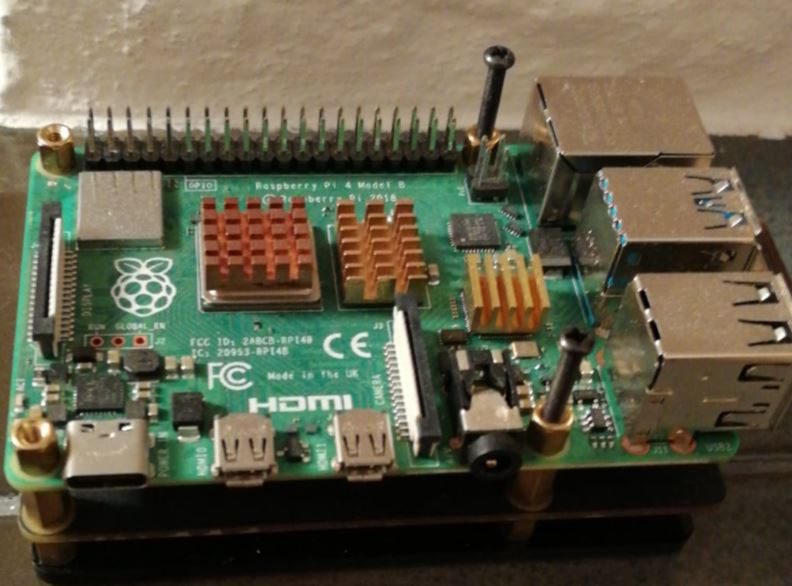
\includegraphics[width=1\textwidth]{pics/Raspberry.JPG}
    \caption{Raspberry Pi des Projektes}
\end{figure}

\subsection{Samba}
Der Raspberry dient weiters als File-Server. Für eine leichtere Datenübertragung zwischen Windows und Linux wird mit Hilfe von Samba über den Windows Explorer direkt auf den Raspberry Pi zugegriffen.
Somit können Files oder Projekte direkt von einem Laptop oder Computer auf den Raspberry PI gelegt werden.

\begin{figure}[H]
    \centering
    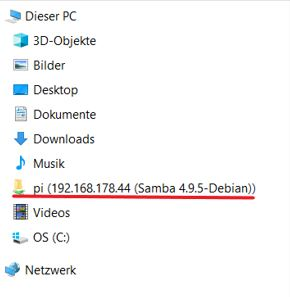
\includegraphics[width=0.5\textwidth]{pics/RaspberrySamba.JPG}
    \caption{Samba auf Laptop}
\end{figure}



\subsection {MQTT auf Raspberry Pi:}
Weiteres dient unser Raspberry auch als MQTT-Broker, welcher Messwerte von Sensoren empfängt und an das Backend, welches als MQTT-Client dient, übermittelt. 
Genaueres wie MQTT aufgebaut ist und in welcher Verbindung der MQTT-Broker zu den MQTT-Clients steht wird im Kapitel MQTT beschrieben.

\subsection {Installation und Verwendung von Docker auf dem Raspberry Pi:}

Docker ist eine Software, welche das Management von Containern übernimmt. Ein Container enthält alle Dateien, die zum Ausführen einer Software notwendig sind. 
Die Installation von Docker wird über ein Skript durchgeführt. 
Dieses wird direkt von Docker zur Verfügung gestellt und führt alle Schritte automatisch ohne weitere Eingaben vom Benutzer durch. 
Nach wenigen Minuten ist Docker betriebsbereit. 
Weiters ist auch eine zentralisierte Servicebereitstellungsplattform für containerisierte Apps 
mit dem Namen Portainer auf dem Raspberry Pi installiert, 
welche eine Liste aller Container und deren Informationen zur Verfügung stellt.
 


\subsection {Remote Access auf einen Raspberry PI:}
Bei Verwendung des Raspberry PI ohne direkt angeschlossenen Monitor kann mittels SSH (Secure Socket Shell) Protokoll von einem Laptop zugegriffen werden.
Dabei muss die IP-Adresse des Raspberry's im Netzwerk bekannt sein. WLAN-Router (FRITZ!Box) bieten über ihre standard IP-Adresse eine Übersicht der verbundenen Geräte, wo auch unter anderem der verbundene Raspberry Pi angezeigt wird. 

 \subsection{Was sind Ip-Adressen:}
Im oberen Kapitel Remote Access ist oft das Wort Ip-Adresse gefallen, deswegen wird in diesem Unterpunkt eine kleine Einführung über Ip-Adressen und Ihre Verwendung gegeben. 
Eine Ip-Adresse ist eine Adresse in Computernetzen, welche von einem Router vergeben wird.
 Einem Gerät kann maximal eine Ip-Adresse zugewiesen werden, jedoch kann die Ip-Adresse auch wechseln, wenn sich das Gerät zum Router erneut verbindet. 
 Im Router gibt es aber auch die Konfigurationsmöglichkeit, dass einem Gerät immer eine bestimmte Ip-Adresse zugewiesen wird.  \cite{RaSPPIInternetZugriff}






\section{MQTT}
\setauthor{Sebastian Egger}

\subsection{Was ist MQTT:}
MQTT ausgeschrieben Message Queuing  Telemetry Transport ist ein Protokoll, welches Nachrichten von einer Maschine zu einer anderen Maschine schickt. 
Ein MQTT Netzwerk besteht  aus mindestens einem MQTT-Broker und zwei MQTT-Clients. 
Wenn ein MQTT-Client eine Message an einen anderen MQTT-Client senden will, muss als erstes eine Message zu dem MQTT-Broker, welcher die Message zu einem sogenannten Topic zuweist, gesendet werden.
Ein Topic ist ein Bereich, wo bestimmte Nachrichten aufgelistet werden. 
Ein Topic in unserem Fall lautet mqtt/noice für den Noice-Sensor.  
Wenn ein oder mehrere MQTT-Clients diese Nachricht empfangen wollen, dann subscriben diese auf das Topic. 
Durch das subscriben von den Clients werden diese, sobald eine neue Message an das Topic gesendet wurde, benachrichtigt und können diese nun empfangen. 
\cite{MQTT}

\subsection {Verwendung von MQTT in unserem Projekt:}
Unser Projekt besteht aus 2 MQTT-Clients und 1 MQTT-Broker. 
Die Sensor Box ist ein MQTT-Client, welcher die Messwerte an den MQTT-Broker sendet. 
Der MQTT-Broker ist im Projekt der Raspberry PI. 
Zum Empfangen der Daten liest das Backend, welches den zweiten MQTT-Client darstellt, die Daten vom Raspberry ein.

\subsection{MQTT-Explorer:}
MQTT-Explorer ist eine kostenlose Software, welches sich für das Testen einer Connection zwischen MQTT-Client und Broker bestens eignet.
Der MQTT-Explorer ist ein weiterer MQTT-Client.
Zur Benutzung und Verbindung mit dem Raspberry ist ein Login mit der Ip-Adresse und Port des Brokers sowie dem dazugehörigen Benutzernamen und Passwort notwendig.

\begin{figure}[H]
    \centering
    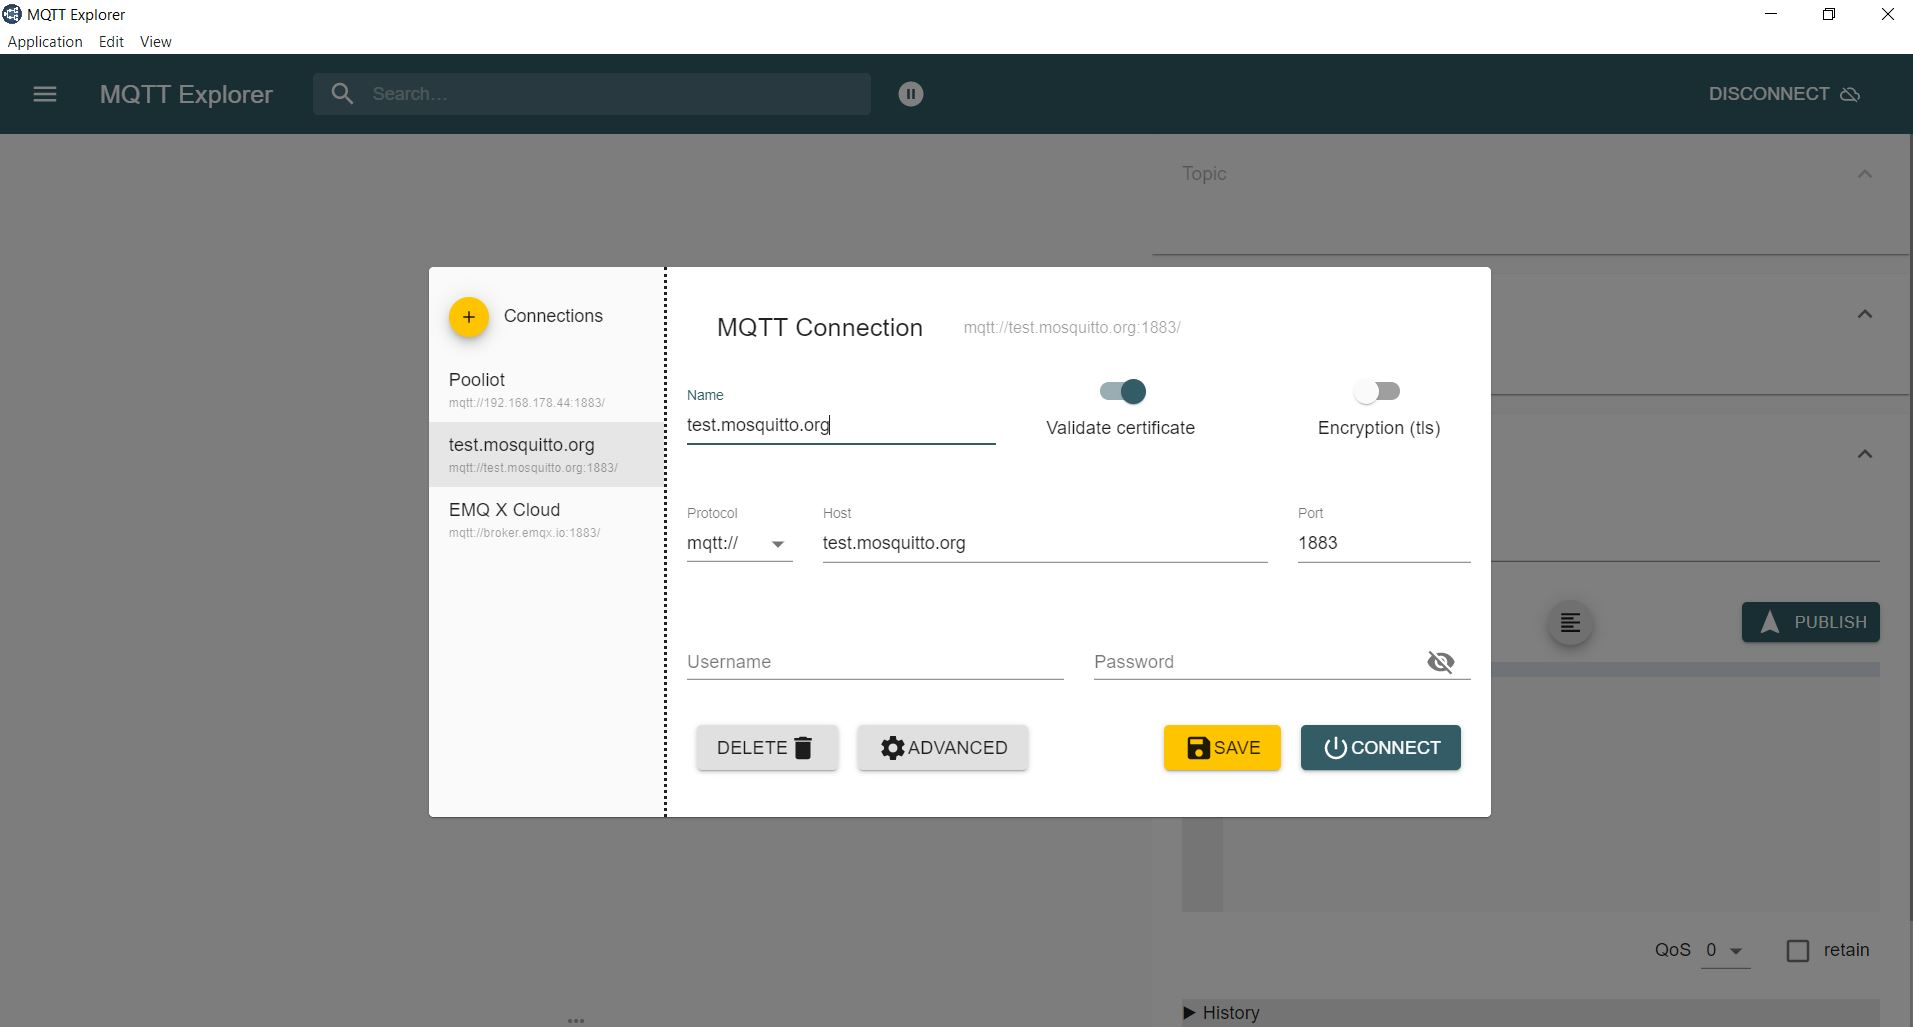
\includegraphics[width=1\textwidth]{pics/MQTTExplorerStartScreen.JPG}
    \caption{MQTT-Explorer Login}
\end{figure}


 Sobald eine Verbindung zu einem MQTT-Broker möglich ist, wird ein Screen mit dem Namen des Brokers und den dazugehörigen Topics aufgelistet. 
 In unten gezeigter Abbildung wurde eine Verbindung mit dem MQTT-Broker test.mosquitto.org hergestellt.  

 \begin{figure}[H]
    \centering
    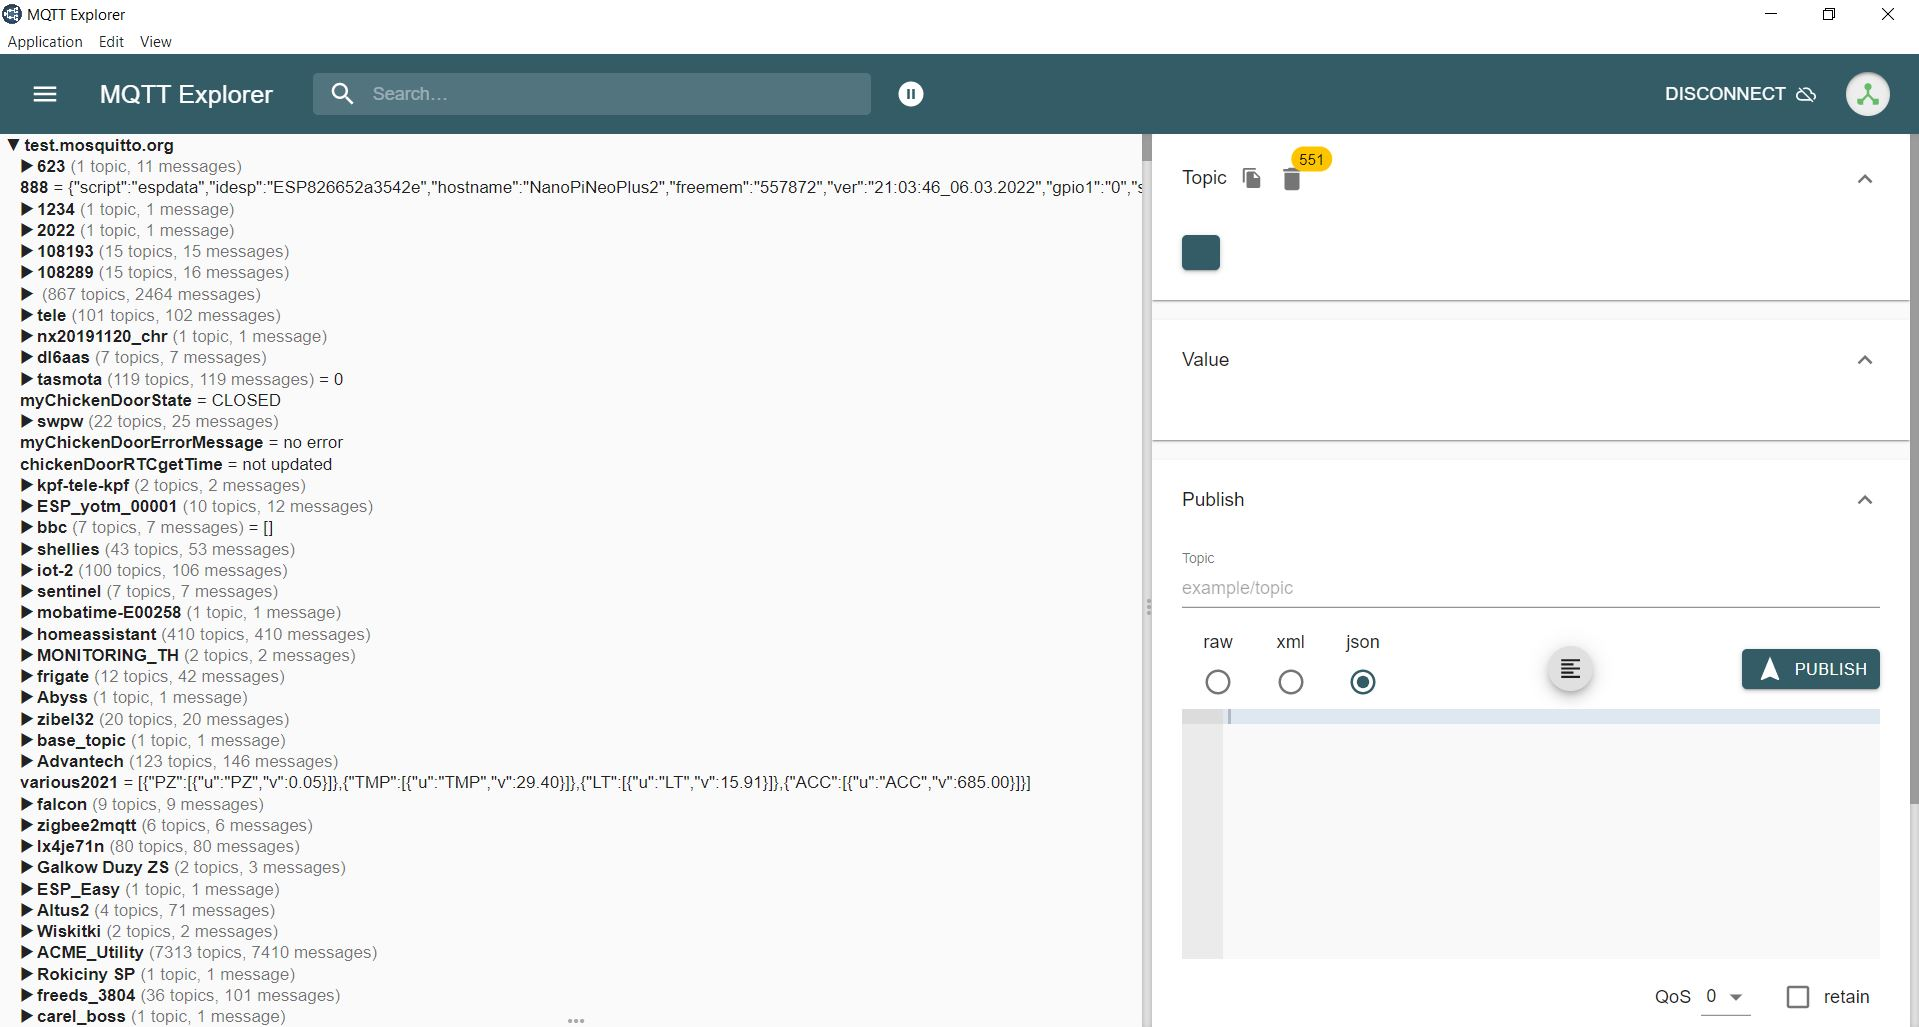
\includegraphics[width=1\textwidth]{pics/MQTTExplorerTestDemo.JPG}
    \caption{MQTT-Explorer nachdem Login}
\end{figure}








\section{.Net}
\setauthor{Sebastian Egger}


\subsection{.Net Core und .Net Framework}

In unserem Projekt verwenden wir .Net Core, eine alternative dazu wäre .NetFramework.
Beides sind Frameworks, welche für die Erstellung serverseitiger Anwendungen verwendet werden. 
.Net Core und .Net Framework haben manche funktionale Komponenten gemeinsam und können Ihren Code auch über die beiden Plattformen hinweg gemeinsam nutzen.

\subsubsection*{ Was wird unter .Net Framework und .Net Core verstanden}
Bisher wurde .NetFramework genützt um sowohl .NET Desktop-Anwendungen als auch serverbasierte Anwendungen zu erstellen.
.NET Core wiederum dient der Erstellung von Serveranwendungen, die unter Windows, Linux und Mac laufen.
Bei .NET Core handelt es sich in erster Linie um ein Open-Source-Framework mit Multiplattform-Unterstützung.
\cite{.NetFrameworkvsCore}

\subsubsection*{.Net Framework Vorteile}
Während .NET Core die Zukunft der Anwendungsentwicklung ist und das .NET Framework in der Zukunft ablösen wird, wird die jahrelange Verwendung von .NET Framework nicht so schnell vergehen!
Spricht man über .NET Framework vs. .NET Core im heutigen Kontext, so hat .NET Framework immer noch einige praktische .NET-Vorteile.

.Net Core benötigt derzeit für unerfahrene Programmierer einen größeren Lernaufwand als bei .Net Framework. 
Ein weiterer Vorteil gegenüber .Net Core ist die Wartung bestehender Anwendungen. 
Nachdem .Net Framework sich seit Jahren im Einsatz befindet, wurden die meisten .Net Anwendungen mittels .Net Framework geschrieben. 
Ein weiterer großer Vorteil von .Net Framework ist die Stabilität der Platform. 

Microsoft hat verkündet, dass die aktuelle Version des Microsoft .NET Frameworks (Version 4.8) die letzte Version sein wird und es danach kein größeres .NET Framework-Update mehr geben wird.
Das bedeutet die Entwicklung von .Net Framework schreitet nicht mehr voran, somit können auch keine durch Updates verursachten Bugs mehr entstehen, aber es gibt keine Garantie, dass neuere 
Betriebssysteme auch in Zukunft .Net Framework noch unterstützen werden. \cite{.NetFramework}

\subsubsection*{.Net Core Vorteile}

Wie bereits oben erwähnt ist .Net Core ein Open-Source-Framework, welches sich kontinuierlich durch offene Beiträge verbessert.
Ein weiterer Vorteil ist die plattformübergreifende Kompatibilität, damit bei Verwendung eines Computers mit Linux oder macOS als Betriebssystem trotzdem Apps, welche unter Windows laufen, verwendet werden können.
Mit .Net Core entwickelten Apps wird Benutzern die Möglichkeit geboten, diese Apps nicht nur unter Windows zu verwenden, sondern auch auf Linux oder macOS. Diese Flexibilität entfällt bei Entwicklungen mit .Net Framework.

Es gibt natürlich noch einige weitere Vorteil von .Net Core, die hier nicht erwähnt wurden.

\subsection{Visual Studio Code}
Visual Studio Code ist ein Code Editor mit vielen Funktionen.
Wie bereits im Kapitel .Net angesprochen, gibt es sehr viele Extensions
in diesem Editor, welche zum Beispiel eine Visualisierung von Inhalten einer Sqlite Datenbank
ermöglicht oder als Latex Editor genutzt werden kann.

\subsection{Visual Studio}
Visual Studio ist ein Code Editor, welcher von Microsoft entwickelt wurde, um eine
benutzerfreundliche Programmierumgebung anzubieten. Seit 2008 wird jedes 
zweite Jahr ein neues Visual Studio mit mehr Funktionen, welche dem Benutzer 
beim Programmieren das Leben vereinfachen, veröffentlicht. 

\subsubsection*{Was ist Swagger und Verwendung von Swagger in unserem Projekt}

Swagger ist eine Sammlung von Open-Source-Werkzeugen, um HTTP-Webservices (auch HTTP API oder REST-like API) zu entwerfen, zu erstellen, 
zu dokumentieren und zu nutzen.
In diesem Projekt wurde Swagger verwendet, um die API zu beschreiben und zu testen.
Swagger bietet nicht nur die Zusammenarbeit mit C\# an sondern auch mit anderen Programmiersprachen wie zum Beispiel
JAVA, JavaScript, Groovy und noch weitere Programmiersprachen, die hier nicht explizit erwähnt werden. 

\subsubsection*{Wie wird ein Swagger in C\# eingebunden}
In C\# kann man Swagger durch ein NuggetPackage Namens Swashbuckle.AspNetCore verwenden.
Durch dieses NuggetPackage kann ein Swagger nun in eine WebApi, wie in nachfolgender Abbildung implementiert werden:


\begin{figure}[H]
    \centering
    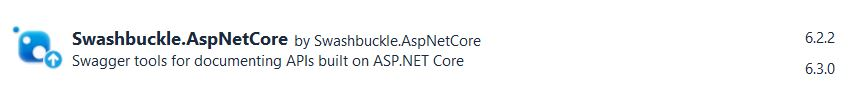
\includegraphics[width=1\textwidth]{./pics/SwaggerNuggetPackage.JPG}
    \caption{DotNet6ConApp}
\end{figure}


Die im Projekt verwendete Implementation wird im Unterkapitel Verwendung von Swagger im Projekt dargestellt.


\subsection {DotNet 5 vs DotNet 6}

Die Entwicklung der Diplomarbeit startete schon mit Sommerbeginn 2021 und .Net6 wurde erst im November 2021 released. 
Aufgrund der schon vorhandenen Kentnisse in .Net5 und der im .Net6 bei Standardkonfiguration nicht vorhandenen Methoden / Usings Unterstützung (siehe nachfolgende Abbildungen)
wurde beschlossen, währen der Umsetzung nicht die Entwicklungsumgebung zu ändern.

Eine Migration von .Net5 auf .Net6 umfasst in der Regel dann das Umstellen aller Paketversionen auf die neueste .NetVersion.
Hier sollten im Bedarfsfall dann nur wenige Änderungen notwendig werden und sollten dann auch aufgrund des längeren Supports von .Net6 
und der Vorteile rund um Performance, die bei eventueller Ausführung in der Cloud sicherlich auch positive Auswirkungen auf die 
Bedarfskosten mit sich bringen kann, in Erwägung gezogen werden.
Persönlich empfundener Nachteil bei der Lesbarkeit des Codes:

\begin{figure}[H]
    \centering
    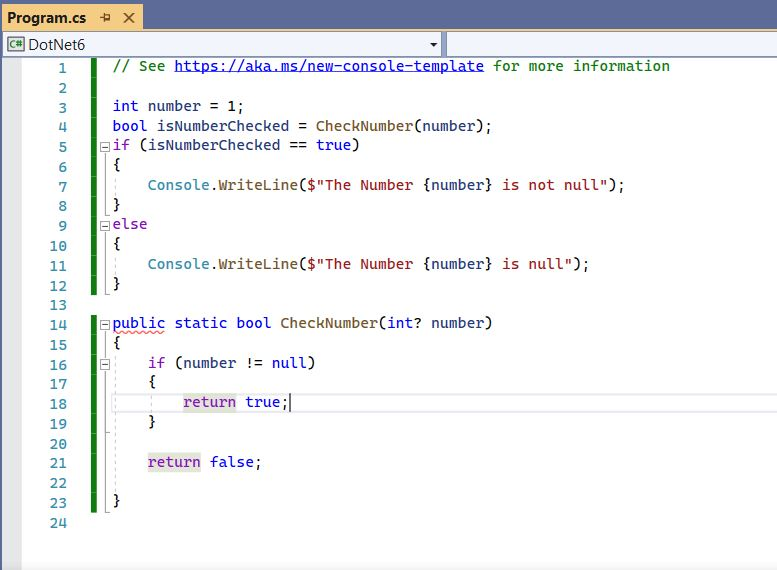
\includegraphics[width=0.7\textwidth]{./pics/DotNet6ConApp.JPG}
    \caption{DotNet6ConApp}
\end{figure}


\begin{figure}[H]
    \centering
    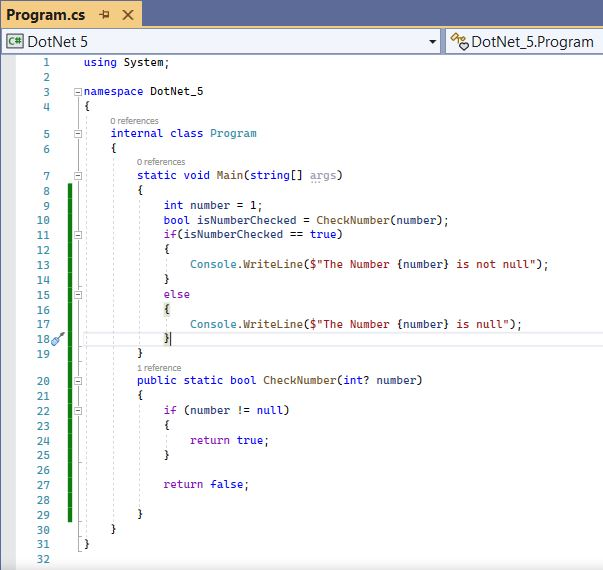
\includegraphics[width=0.7\textwidth]{./pics/DotNet5ConApp.JPG}
    \caption{DotNet5ConApp}
\end{figure}


Im Vergleich zu .Net6 ist die Unterstützung bei der Verwendung von Usings und Methoden unter .Net5 klar zu erkennen.
\cite{.Net6}

\subsubsection*{Was ist eine Datenbank und wofür eignet sich eine Datenbank}
Eine Datenbank ist eine Sammlung von strukturierten Informationen oder Daten, die typischerweise elektronisch in einem Computersystem gespeichert sind.
Solch eine Datenbank wird meistens von einem Datenbankverwaltungssystem abgekürzt DBMS gesteuert und sie besteht aus Tabellen, in welchen die Daten gespeichert sind.
Auf diese gespeicherten Daten kann mittels SQL-Abfragen zugegriffen werden.
\cite{Database}


\subsubsection*{Warum Sqlite und nicht SqlServer als Datenbank:}

In diesem Projekt wird eine Sqlite-Datenbank verwendet, weil die Datenbank im Vergleich zu einem Microsoft SQL Server eine kleinere
Version ist und sich sehr gut für Endgeräte eignet, da der Raspberry Pi nur über einen begrenzten Speicher verfügt.
Weiters muss auch Rücksicht auf die Architektur vom ARM genommen werden, denn die Version muss für die CPU Architektur geeignet sein.
Hinweis: Microsoft stellte erst mit SQL Server 2017 die erste Version auf Linux zur Verfügung, aber erst mit der Version 2019 sind die meisten
Funktionen wie unter Windows verfügbar.

\subsubsection*{Überprüfung einer Sqlite Datenbank}
Zum Überprüfen einer Sqlite Datenbank eignet sich in Visual Studio Code die Extension "SQLite", 
welche das Innenleben einer SQLite Datenbank veranschaulicht.

\begin{figure}[H]
    \centering
    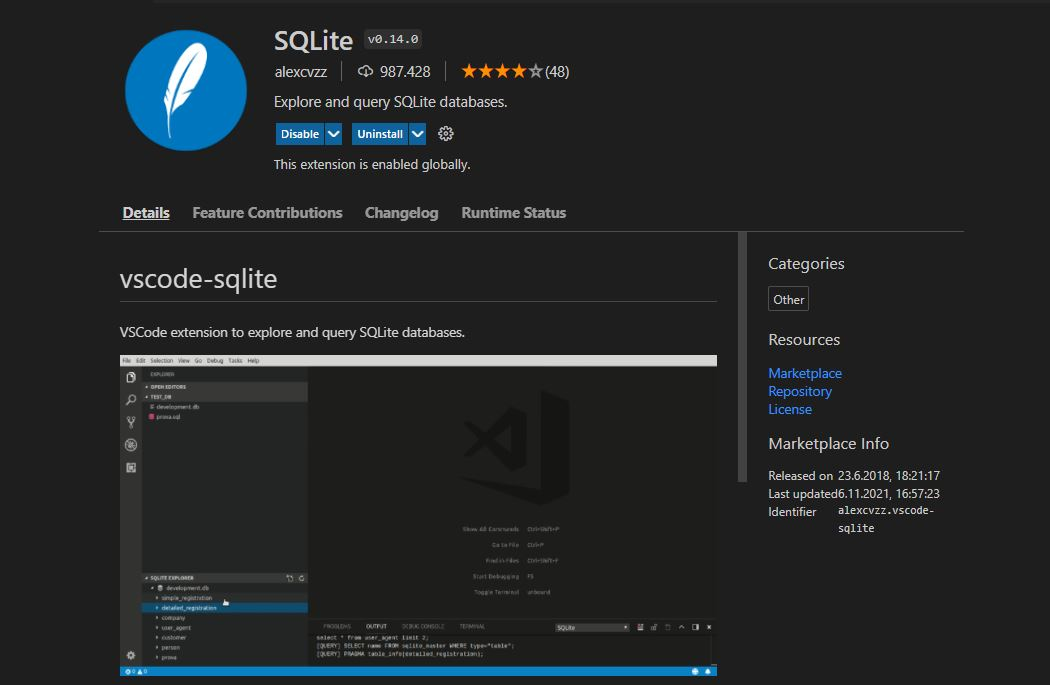
\includegraphics[width=0.8\textwidth]{./pics/SQLiteVSCodeExtension.JPG}
    \caption{SQLite Extension für Visual Studio Code}
\end{figure}

\begin{figure}[H]
    \centering
    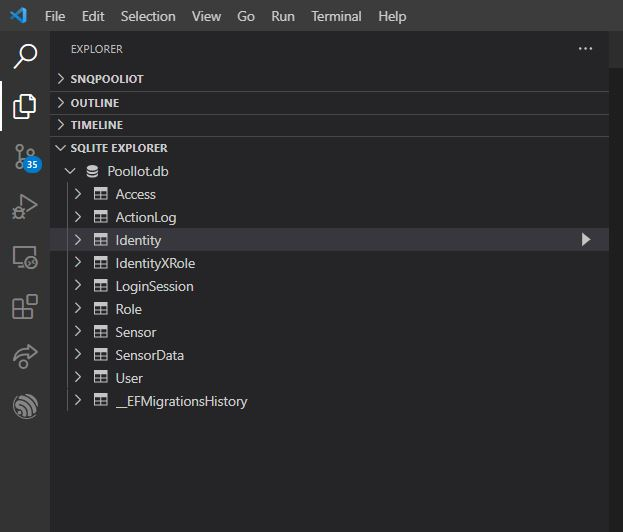
\includegraphics[width=0.8\textwidth]{./pics/SQLiteDatabaseStructure.JPG}
    \caption{Innenleben der SQLite Datenbank}
\end{figure}



\subsubsection*{Asynchrone Programmierung und Implementierung in C\#}
Es sollte wenn möglich immer asynchron programmiert werden, weil es Zeit spart, denn Prozesse können dadurch parallel ausgeführt werden.
Somit muss ein Prozess nicht mehr auf einen anderen Prozess warten.
Ein kleines Beispiel hierfür wäre ein Frühstück, denn eine Person muss eben nicht warten bis das Toastbrot fertig ist, um sich danach erst den Kaffee zu machen, dieses Tun sollte parallel möglich sein.

In C\# gibt es die Keywörter async und await. Wenn eine Methode asynchron aufgerufen werden soll, muss die Methode im Methodenkopf als Kennung async aufweisen und einen Task als return Wert festlegen.
Um diese Methode danach aufrufen zu können, muss await vor dem Methodennamen verwendet werden.
\cite{Async}

\subsubsection*{Keyword partial C\#}
In C\# gibt es das sogenannte Keyword partial, wodurch die Implementierung von einer Methode in einer Klasse der selben Klasse jedoch in einem anderen File passieren kann.
Ein Code Beispiel im Projekt wäre die SnQPoolIot.ConApp.

In den nachstehenden 2 Abbildungen wird beschrieben wie eine Implementierung von einer partial Method erfolgt.

Im ersten Foto ist zu erkennen, dass die Klasse Program.cs partial gesetzt wurde und die Methode BeforeRun() auch das Keyword partial beinhaltet.
\begin{figure}[H]
    \centering
    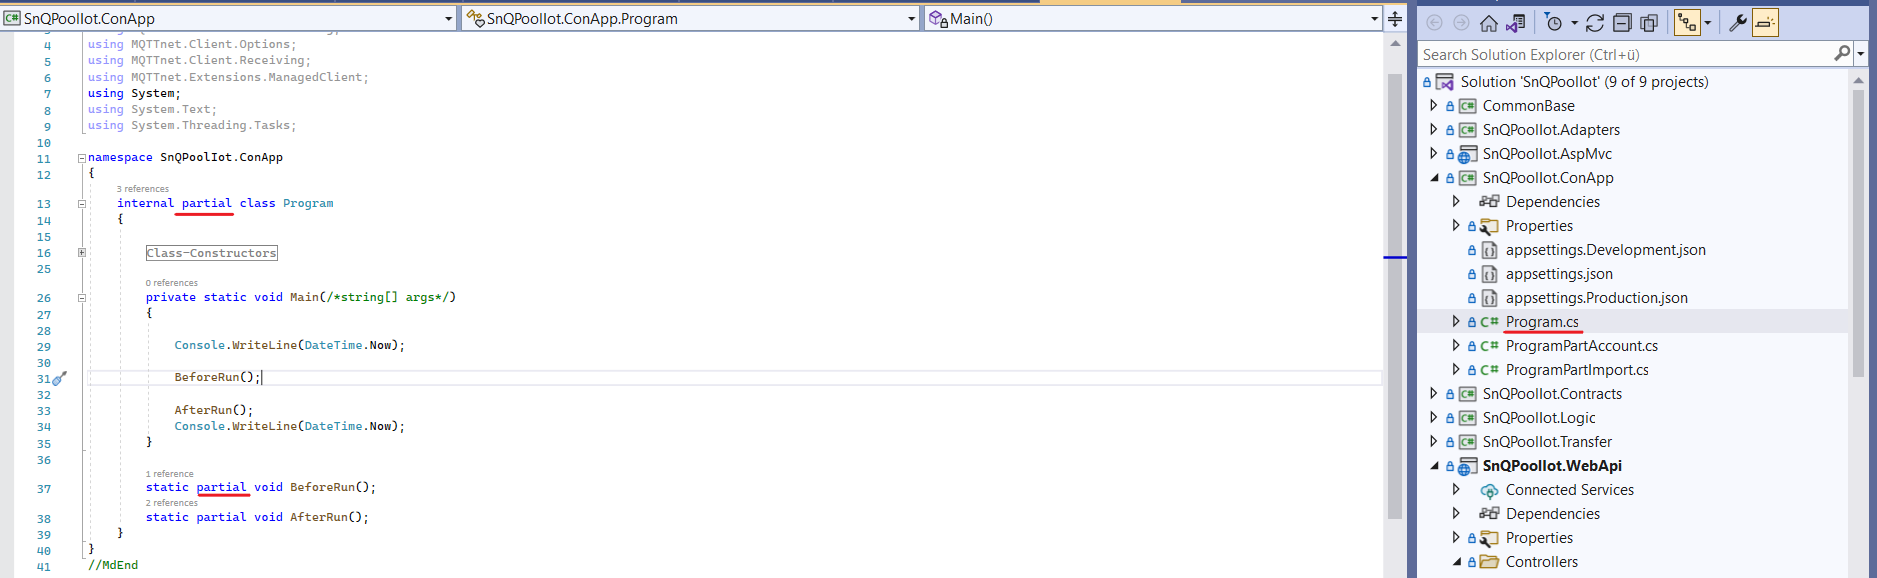
\includegraphics[width=1\textwidth]{./pics/PartialKeyword1.png}
    \caption{Implementierung partial Class und Method}
\end{figure}

Für die Implementierung in einem anderen File wird der Name des Files auf einen anderen Namen umbenannt und danach wird die Klasse wieder auf Programm.cs umgeschrieben.
Nun erkennt C\# das es sich um eine partial Class handelt und somit können nun die Methoden, welche in der Klasse partial sind, aber in einem anderen File liegen, umgeschrieben werden. 
\begin{figure}[H]
    \centering
    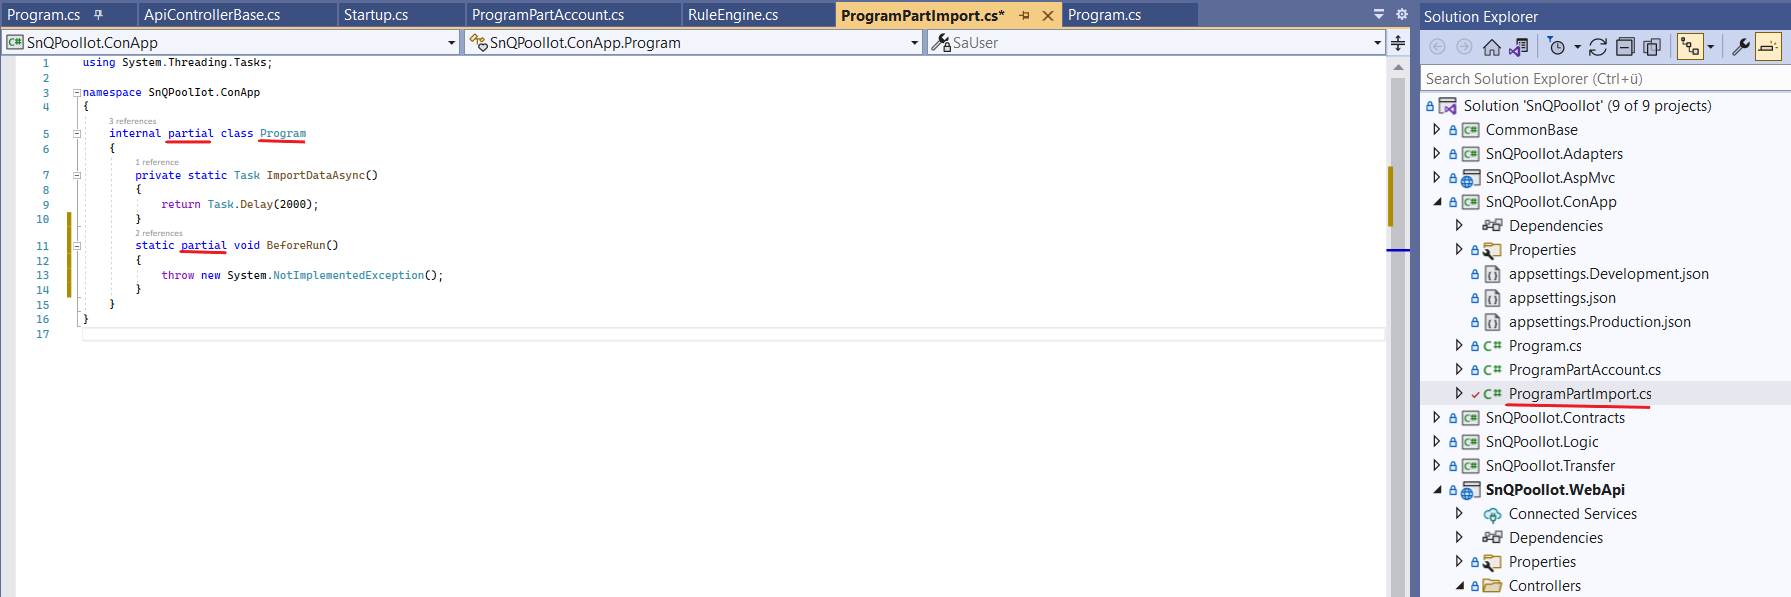
\includegraphics[width=1\textwidth]{./pics/PartialKeyword2.png}
    \caption{Implementierung partial Class und Method}
\end{figure}
\cite{KeywordPartial}

\section{Telegram}
\setauthor{Sebastian Egger}
Telegram ist ein Messaging-Dienst wie WhatsApp, welcher auf Smartphones und Computer vorzufinden ist.
In diesem Projekt wird Telegram auch zum Versenden und Empfangen von Messages verwendet, jedoch über einen sogenannten Bot.
Telegram hat ein eigenes Botnetzwerk, wodurch Messages über das Internet gesendet werden können.
Um einen Bot für solche Zwecke erzeugen zu können, muss bei dem sogenannten BotFather ein Bot erzeugt werden.

\begin{figure}[H]
    \centering
    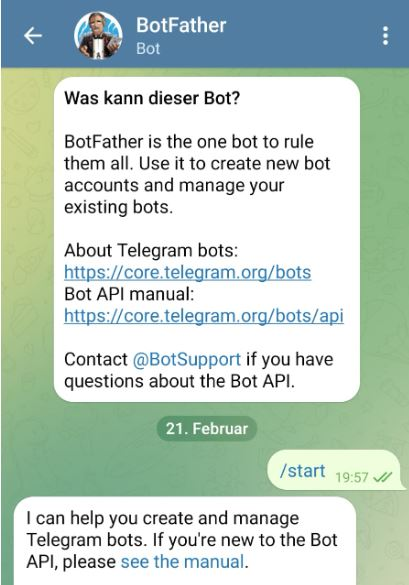
\includegraphics[width=0.8\textwidth]{./pics/BotFather.JPG}
    \caption{Erzeugen eines Bots über den BotFather}
\end{figure}

Sobald der BotFather gestartet wurde, kann über den Befehl /newbot ein neuer Bot erzeugt 
werden, indem eine Person dem Bot einen Namen und einen nicht existenten Usernamen,der mit bot endet, zuweist.
Wenn dieser Vorgang durchgeführt wurde, kann auf den Bot über HTTP Requests zugegriffen werden.

\begin{figure}[H]
    \centering
    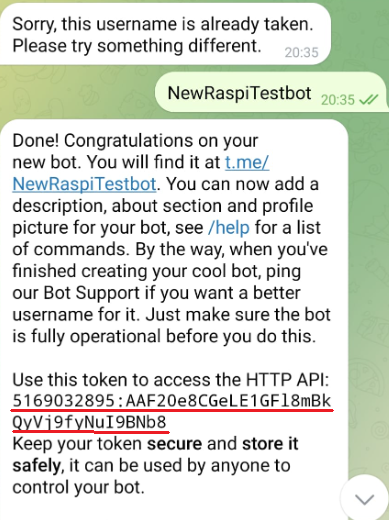
\includegraphics[width=0.8\textwidth]{./pics/TelegramBotCreatedToken.png}
    \caption{Beispiel eines Tokens der zum Zugriff auf die API benötigt wird.}
\end{figure}

Durch diesen Token kann über das Internet Messages gesendet werden oder auch die ChatId, welche
eine große Rolle im Backend des Projektes spielt, herausfinden. Der Befehl um die ChatId zu erlangen lautet:

https://api.telegram.org/bot(Token)/getMe 
\\danach kann eine Message über den Befehl \\
https://api.telegram.org/bot(Token)/sendMessage?chat\_id=(chatId)\&text=\"Text\" ddddddd 
\\gesendet werden.

\section{Begriffserklärungen}

\subsection{C\#}
C\# ist eine objektorentierte Programmiersprache, welche von Microsoft entwickelt
wurde

\subsection{ARM}
ARM stand für Acorn RISC Machines, später für Advanced RISC Machines 
und ist einer der meistverbreiteten Mikroprozessoren.
